\chapter{Results}\label{chap:results}
\section{Results for titles generations}
To evaluate the performance of the model in automatically generating pull request messages, three metrics were used: BLEU, METEOR, and cosine similarity. Violin plots provide a visual representation of the distribution of scores obtained for each experimental configuration, labeled as first, second, third, and fourth.
\begin{figure}[H] 
    \centering
        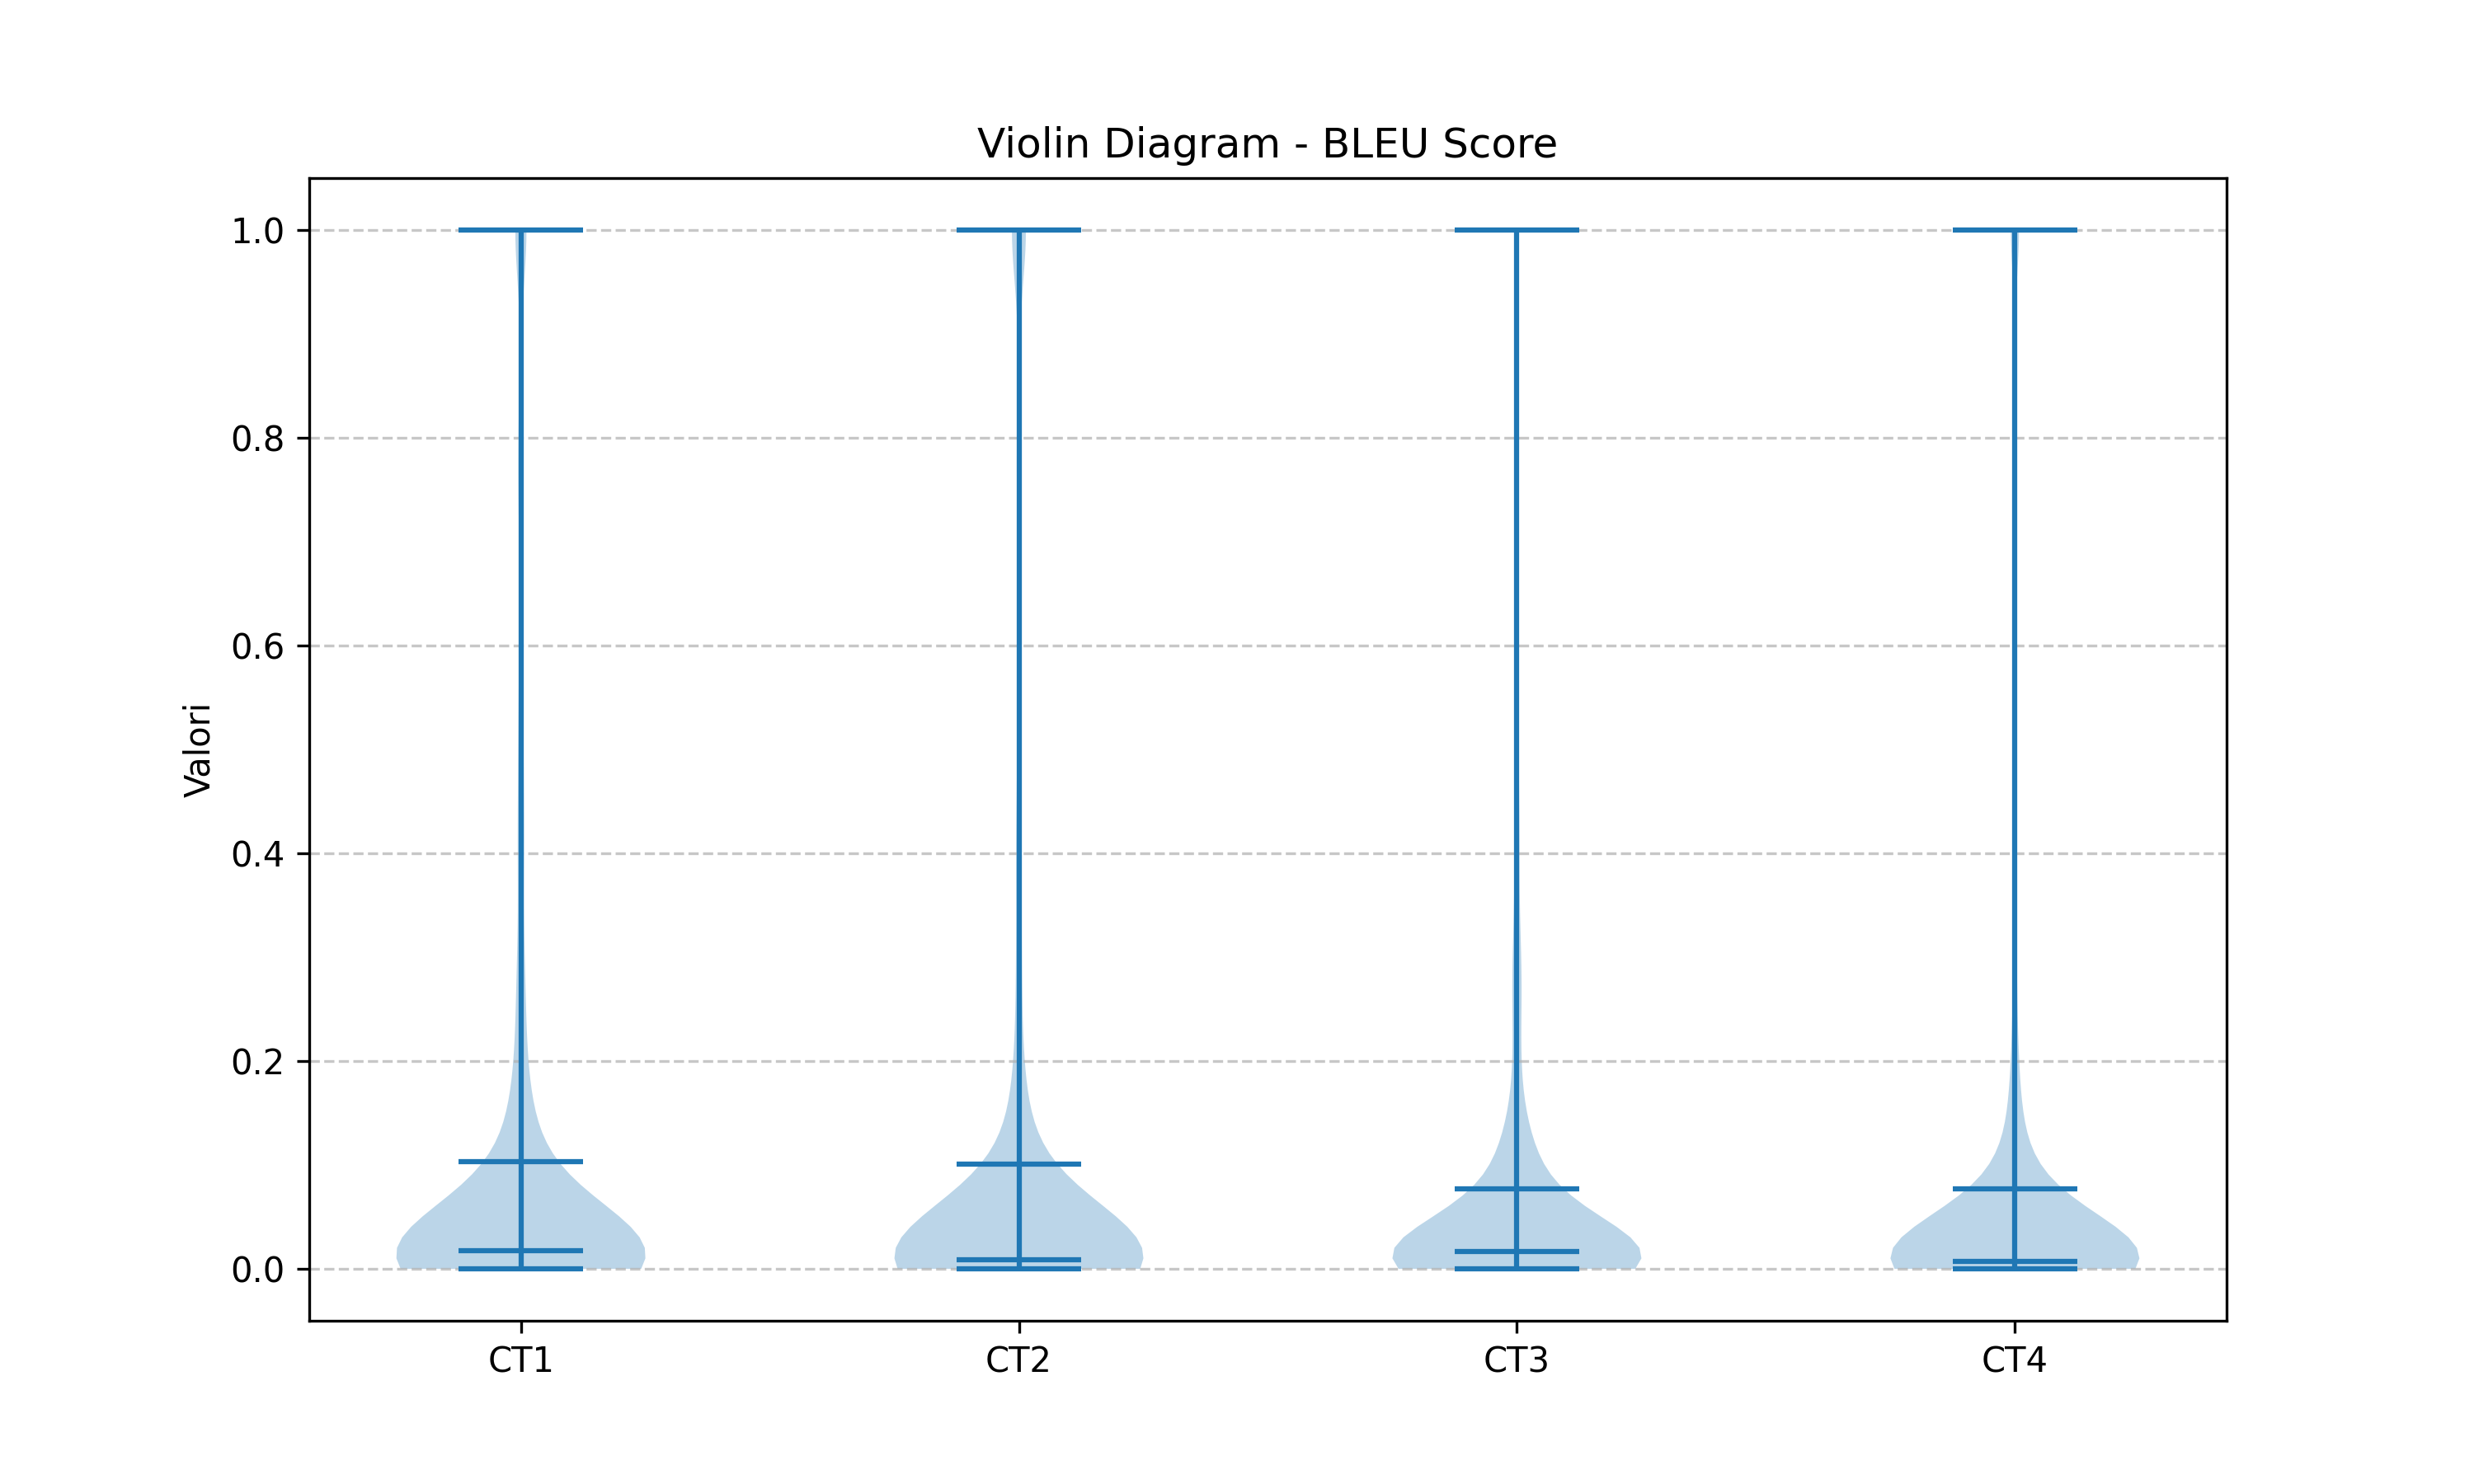
\includegraphics[width=\linewidth]{figures/violin_bleu.png}
        \caption{Distribution of BLEU scores for different experiment configurations.}
\end{figure}
The violin plot for the BLEU metric shows a highly concentrated distribution toward values close to zero, with a few exceptions reaching high values up to 1.0. This indicates that most generations have a low n-gram correspondence with the reference titles, suggesting that the model struggles to exactly replicate the word sequences. However, the presence of some high-scoring outliers suggests that, in specific cases, the model was able to generate titles very similar to the original ones.
\begin{figure}[H]
    \centering
        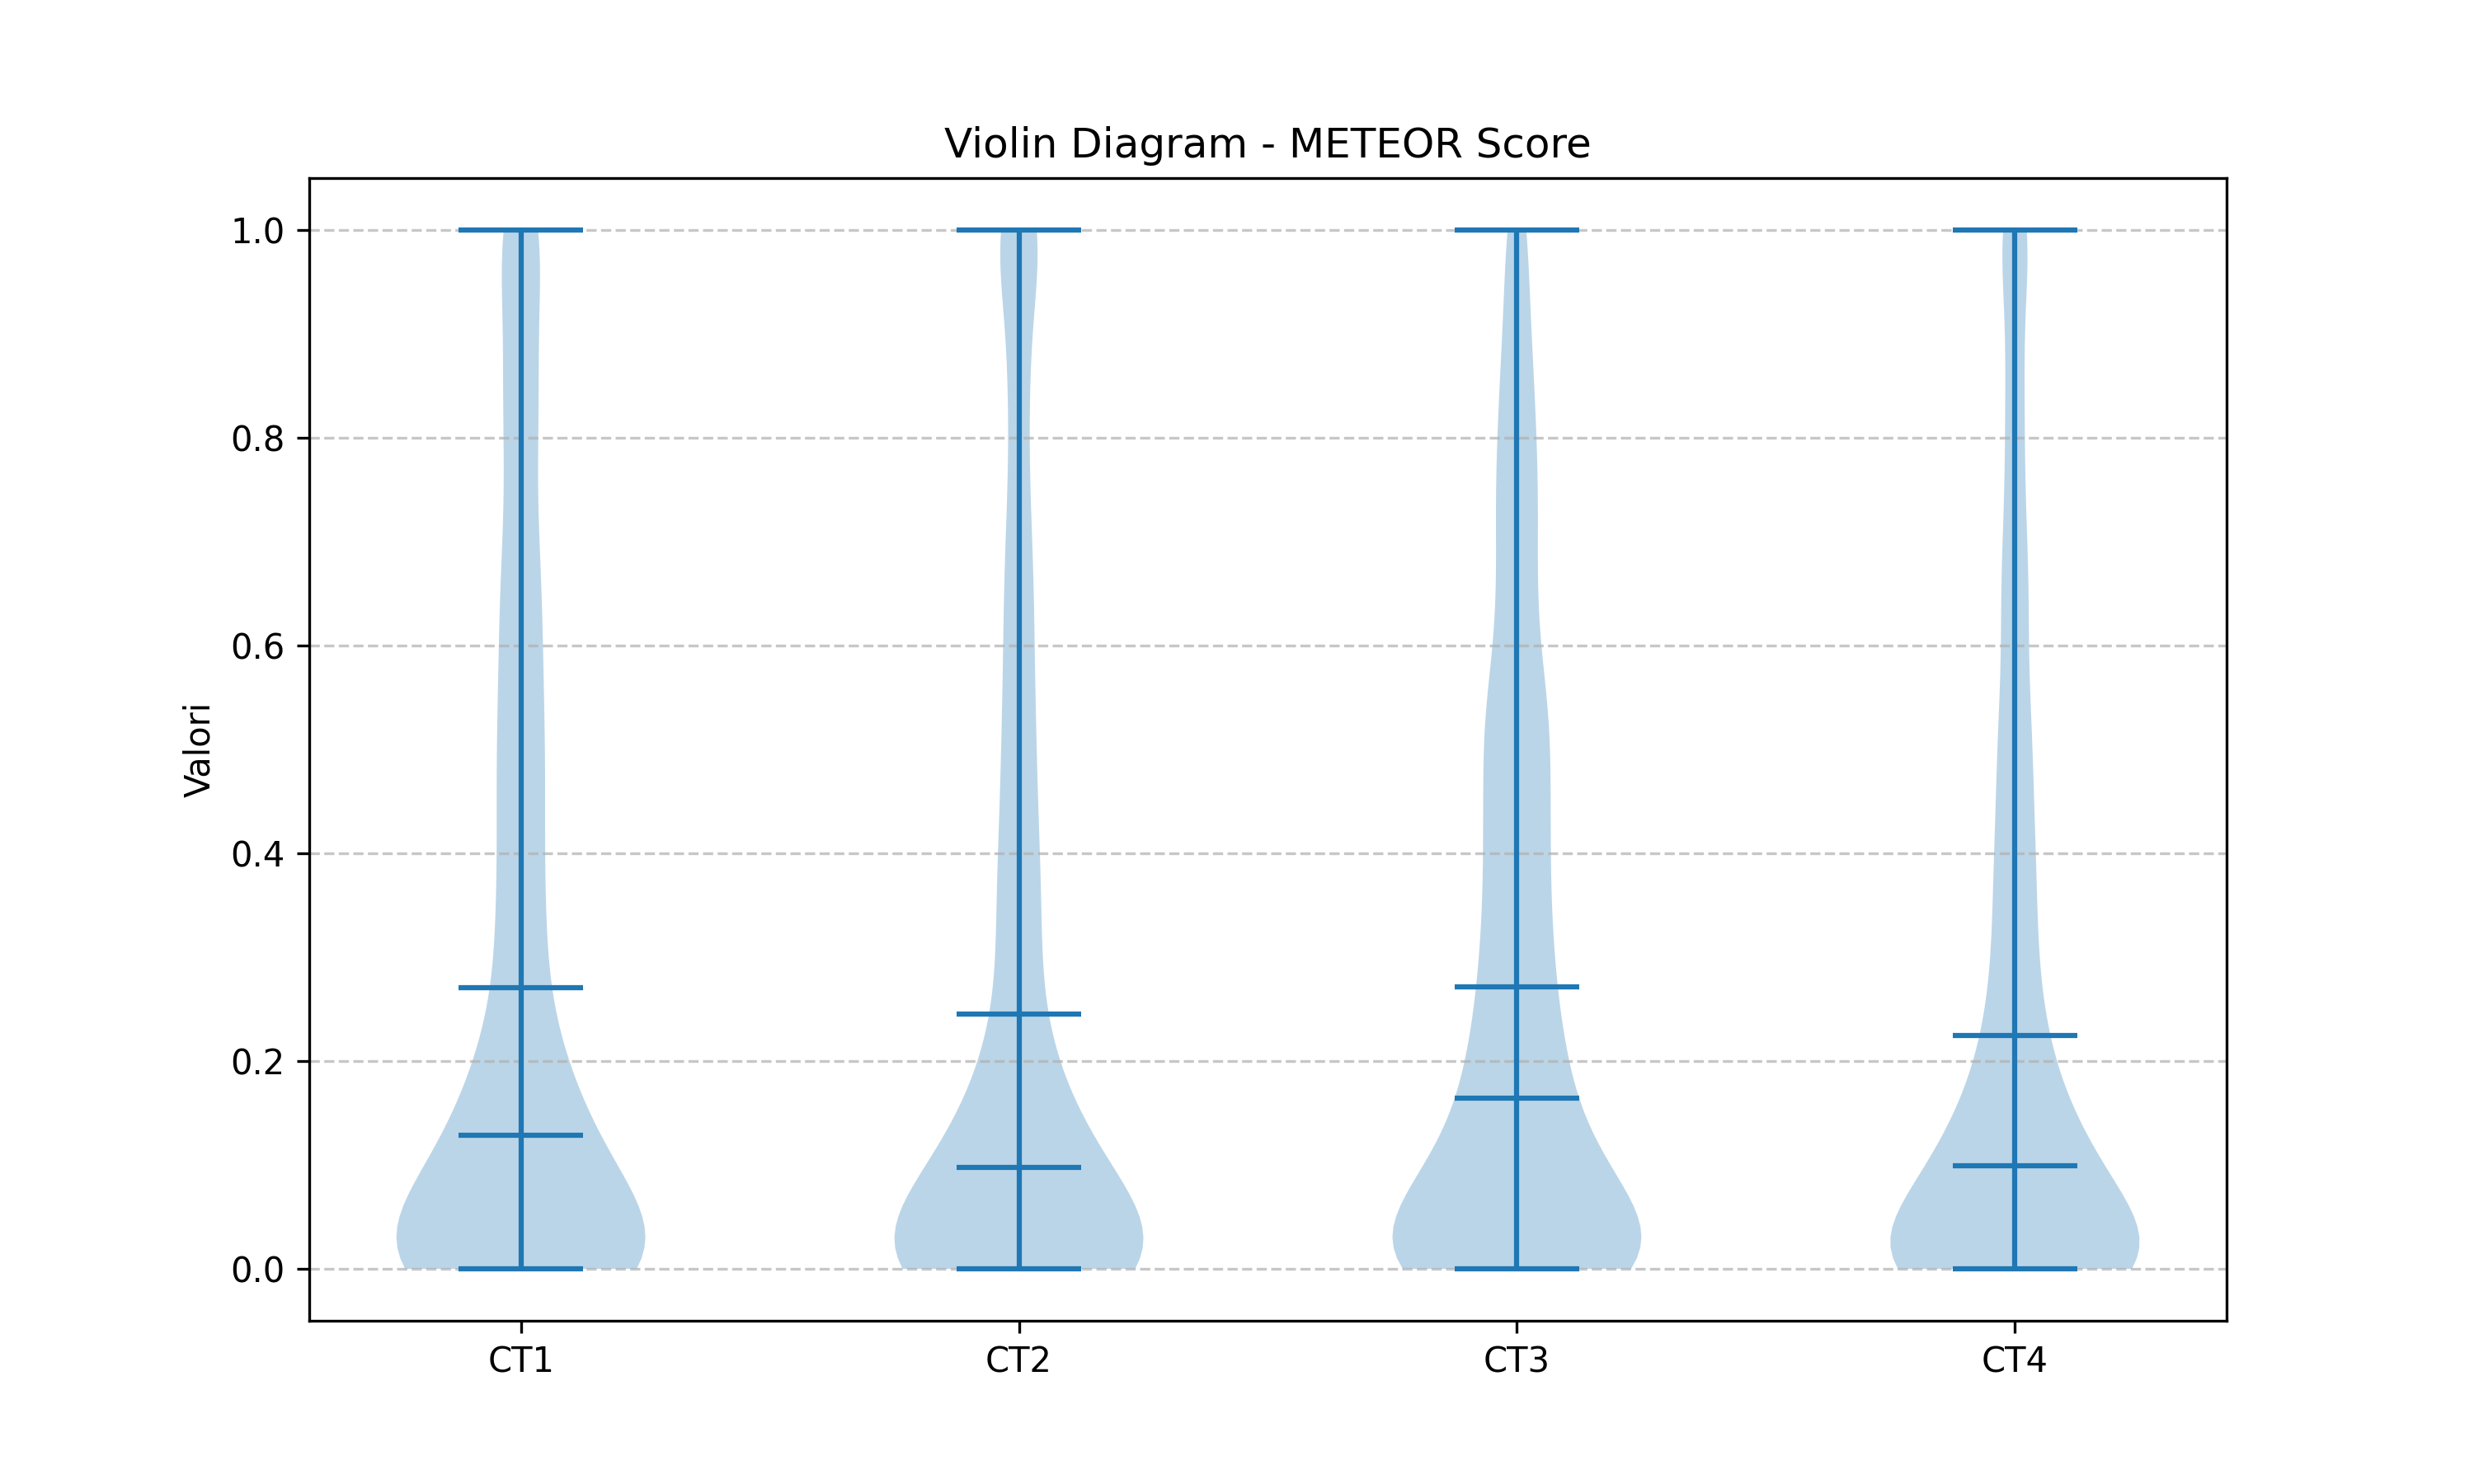
\includegraphics[width=\linewidth]{figures/violin_meteor.png}
        \caption{Distribution of METEOR scores for different experiment configurations.}
\end{figure}
The METEOR diagram shows a distribution similar to that of BLEU, with most scores concentrated on low values, but with greater variability. Some outliers reach values close to 1.0, indicating that the model has generated titles very aligned with the reference ones in terms of lexical and semantic correspondence. Compared to BLEU, METEOR tends to be more generous with lexical variations, which explains the greater dispersion of scores.
\begin{figure}[H] 
    \centering
        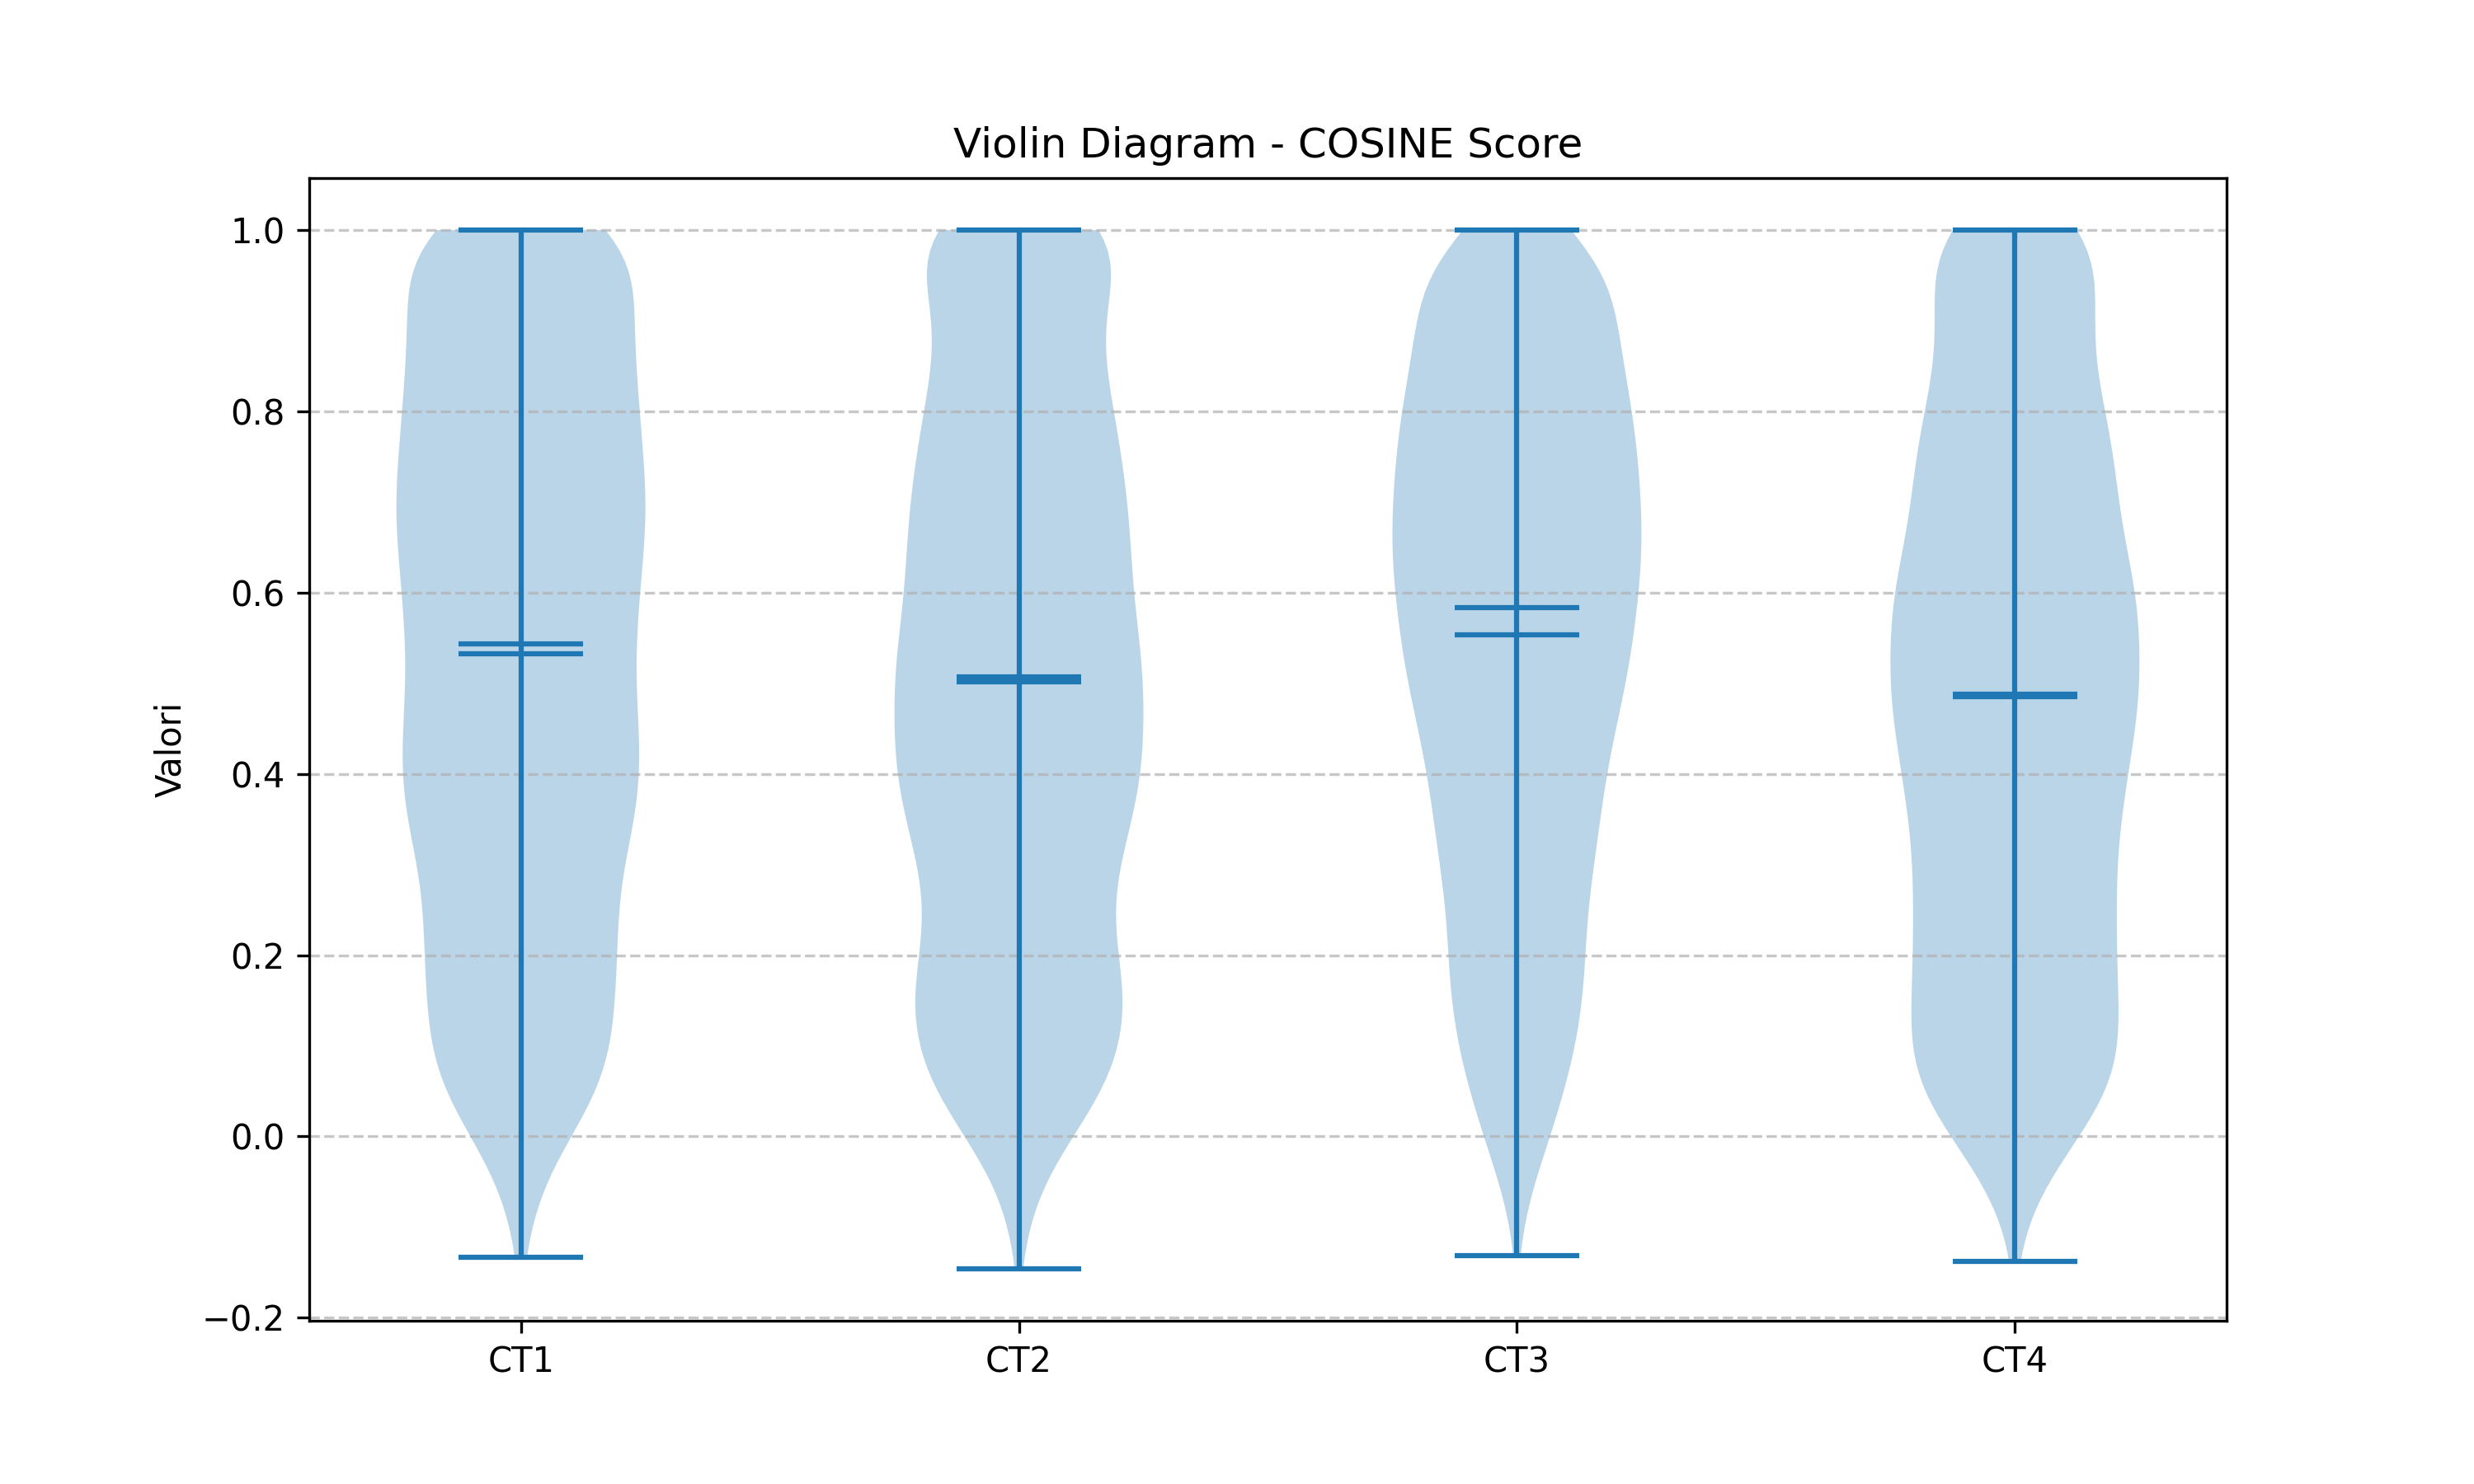
\includegraphics[width=\linewidth]{figures/violin_cosine.png}
        \caption{Distribution of cosine similarity scores for different experiment configurations.}
\end{figure}
The cosine similarity plot shows a more uniform distribution than BLEU, with values ranging from about -0.1 to 1.0. The highest density is observed at average values between 0.4 and 0.6, indicating a moderate semantic similarity between the generated and reference titles. This suggests that, while not replicating the same words exactly (as evidenced by the low BLEU scores), the model manages to maintain a certain semantic coherence.
\subsection{Considerations}
The results suggest that the model has a good ability to generate semantically coherent titles, as evidenced by the cosine similarity scores. However, the low lexical adherence detected by BLEU and METEOR indicates room for improvement in the model's ability to reproduce the exact structures of the target titles. The differences between the experimental configurations do not seem particularly marked, suggesting that further optimizations of the prompt or of the model architecture may be necessary to obtain significant improvements.
\section{Results for body message generations}